\documentclass[border=5pt]{standalone}
\usepackage{tikz}
\usepackage{pgfplots}
\pgfplotsset{compat=1.18}
\usepgfplotslibrary{colormaps}

\begin{document}

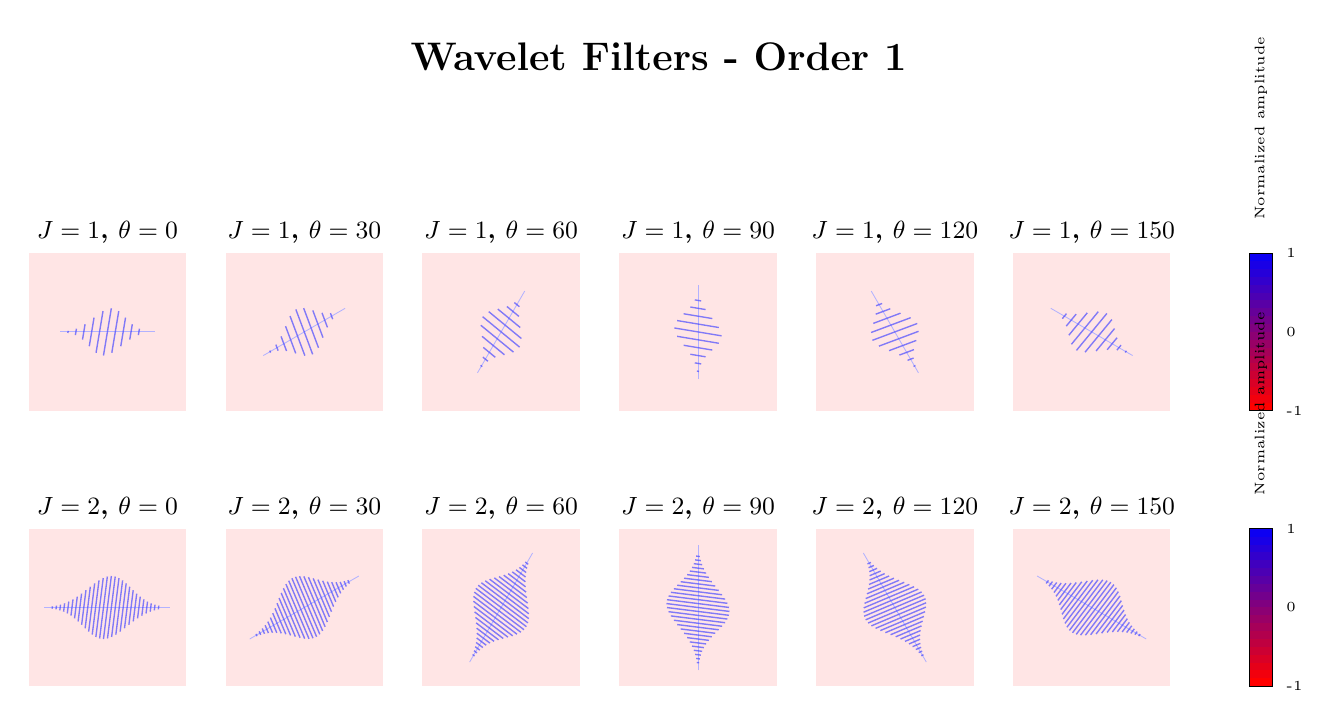
\begin{tikzpicture}
    % Title
    \node[font=\Large\bfseries] at (8, 11.5) {Wavelet Filters - Order 1};
    
    % Define scales and orientations
    \pgfmathsetmacro{\boxwidth}{2}
    \pgfmathsetmacro{\boxheight}{2}
    \pgfmathsetmacro{\xspacing}{2.5}
    \pgfmathsetmacro{\yspacing}{3}
    
    % First row: J = 1
    \foreach \angle/\col in {0/0, 30/1, 60/2, 90/3, 120/4, 150/5} {
        \pgfmathsetmacro{\xpos}{\col * \xspacing}
        \pgfmathsetmacro{\ypos}{7}
        
        % Draw the box with Morlet wavelet
        \begin{scope}[shift={(\xpos, \ypos)}]
            % Background
            \fill[red!10] (0,0) rectangle (\boxwidth, \boxheight);
            
            % Title
            \node[above, font=\small\bfseries] at (\boxwidth/2, \boxheight) {$J = 1$, $\theta = \angle°$};
            
            % Draw simplified Morlet wavelet representation
            \begin{scope}[shift={(\boxwidth/2, \boxheight/2)}]
                % Gaussian envelope (ellipse)
                \draw[blue!30, line width=0.3pt] 
                    plot[domain=-0.6:0.6, samples=50, smooth] 
                    ({cos(\angle)*\x - sin(\angle)*0}, {sin(\angle)*\x + cos(\angle)*0});
                
                % Oscillations inside
                \foreach \t in {-0.5, -0.4, ..., 0.5} {
                    \pgfmathsetmacro{\amp}{exp(-(\t*\t)/0.08)}
                    \draw[blue!70, line width=0.5pt, opacity=0.7] 
                        ({cos(\angle)*(\t-0.05*\amp) - sin(\angle)*(-0.3*\amp)}, 
                         {sin(\angle)*(\t-0.05*\amp) + cos(\angle)*(-0.3*\amp)}) --
                        ({cos(\angle)*(\t+0.05*\amp) - sin(\angle)*(0.3*\amp)}, 
                         {sin(\angle)*(\t+0.05*\amp) + cos(\angle)*(0.3*\amp)});
                }
            \end{scope}
        \end{scope}
    }
    
    % Second row: J = 2
    \foreach \angle/\col in {0/0, 30/1, 60/2, 90/3, 120/4, 150/5} {
        \pgfmathsetmacro{\xpos}{\col * \xspacing}
        \pgfmathsetmacro{\ypos}{3.5}
        
        % Draw the box with Morlet wavelet
        \begin{scope}[shift={(\xpos, \ypos)}]
            % Background
            \fill[red!10] (0,0) rectangle (\boxwidth, \boxheight);
            
            % Title
            \node[above, font=\small\bfseries] at (\boxwidth/2, \boxheight) {$J = 2$, $\theta = \angle°$};
            
            % Draw simplified Morlet wavelet representation (larger scale)
            \begin{scope}[shift={(\boxwidth/2, \boxheight/2)}]
                % Gaussian envelope (larger ellipse)
                \draw[blue!30, line width=0.3pt] 
                    plot[domain=-0.8:0.8, samples=50, smooth] 
                    ({cos(\angle)*\x - sin(\angle)*0}, {sin(\angle)*\x + cos(\angle)*0});
                
                % More oscillations (smaller frequency)
                \foreach \t in {-0.7, -0.65, ..., 0.7} {
                    \pgfmathsetmacro{\amp}{exp(-(\t*\t)/0.15)}
                    \draw[blue!70, line width=0.5pt, opacity=0.7] 
                        ({cos(\angle)*(\t-0.05*\amp) - sin(\angle)*(-0.4*\amp)}, 
                         {sin(\angle)*(\t-0.05*\amp) + cos(\angle)*(-0.4*\amp)}) --
                        ({cos(\angle)*(\t+0.05*\amp) - sin(\angle)*(0.4*\amp)}, 
                         {sin(\angle)*(\t+0.05*\amp) + cos(\angle)*(0.4*\amp)});
                }
            \end{scope}
        \end{scope}
    }
    
    % Colorbar for first row
    \begin{scope}[shift={(15.5, 7)}]
        \foreach \y in {0, 0.1, ..., 2} {
            \pgfmathsetmacro{\val}{(\y/2)*2 - 1}
            \pgfmathsetmacro{\colval}{(\y/2)*100}
            \fill[blue!\colval!red] (0, \y) rectangle (0.3, \y+0.1);
        }
        \draw (0, 0) rectangle (0.3, 2);
        \node[right, font=\tiny] at (0.35, 2) {1};
        \node[right, font=\tiny] at (0.35, 1) {0};
        \node[right, font=\tiny] at (0.35, 0) {-1};
        \node[right, font=\tiny, rotate=90] at (0.15, 2.3) {Normalized amplitude};
    \end{scope}
    
    % Colorbar for second row
    \begin{scope}[shift={(15.5, 3.5)}]
        \foreach \y in {0, 0.1, ..., 2} {
            \pgfmathsetmacro{\val}{(\y/2)*2 - 1}
            \pgfmathsetmacro{\colval}{(\y/2)*100}
            \fill[blue!\colval!red] (0, \y) rectangle (0.3, \y+0.1);
        }
        \draw (0, 0) rectangle (0.3, 2);
        \node[right, font=\tiny] at (0.35, 2) {1};
        \node[right, font=\tiny] at (0.35, 1) {0};
        \node[right, font=\tiny] at (0.35, 0) {-1};
        \node[right, font=\tiny, rotate=90] at (0.15, 2.3) {Normalized amplitude};
    \end{scope}
    
\end{tikzpicture}

\end{document}